% Using mnras_template.tex
%
% LaTeX template for creating an MNRAS paper
%
% v3.0 released 14 May 2015
% (version numbers match those of mnras.cls)
%
% Copyright (C) Royal Astronomical Society 2015
% Authors:
% Keith T. Smith (Royal Astronomical Society)

%%%%%%%%%%%%%%%%%%%%%%%%%%%%%%%%%%%%%%%%%%%%%%%%%%
\documentclass[fleqn,usenatbib]{mnras}
\usepackage[T1]{fontenc}

% Allow "Thomas van Noord" and "Simon de Laguarde" and alike to be sorted by "N" and "L" etc. in the bibliography.
% Write the name in the bibliography as "\VAN{Noord}{Van}{van} Noord, Thomas"
\DeclareRobustCommand{\VAN}[3]{#2}
\let\VANthebibliography\thebibliography
\def\thebibliography{\DeclareRobustCommand{\VAN}[3]{##3}\VANthebibliography}

%%%%% AUTHORS - PLACE YOUR OWN PACKAGES HERE %%%%%
\usepackage{graphicx}	% Including figure files
\usepackage{amsmath}	% Advanced maths commands
\usepackage{amssymb}	% Extra maths symbols

%%%%%%%%%%%%%%%%%%%%%%%%%%%%%%%%%%%%%%%%%%%%%%%%%%

%%%%% AUTHORS - PLACE YOUR OWN COMMANDS HERE %%%%%


\newcommand{\vdag}{(v)^\dagger}
\newcommand\latex{La\TeX}
\newcommand{\Msun}{\,{\rm M}$_{\odot}$\,}
\newcommand{\Msunh}{\,{\rm M}$_{\odot}$\,\,\ifmmode h^{-1}\else $h^{-1}$\fi}
\newcommand{\kms}{\,{\rm km s}\ifmmode ^{-1}\,\else $^{-1}$\,\fi}
\newcommand{\Mpch}{\,{\rm Mpc}\,\ifmmode h^{-1}\else $h^{-1}$\fi}
\newcommand{\kpch}{\,{\rm kpc}\,\ifmmode h^{-1}\else $h^{-1}$\fi}
\newcommand{\kpc}{\,{\rm kpc}\,}

%%%%%%%%%%%%%%%%%%%%%%%%%%%%%%%%%%%%%%%%%%%%%%%%%%

%%%%%%%%%%%%%%%%%%% TITLE PAGE %%%%%%%%%%%%%%%%%%%

\title[Cosmic Web Graph Complexity]{The complexity of the cosmic web graph}

\author[Torres-Guar\'in et al.]{
D. A. Torres-Guar\'in,$^{1}$\thanks{E-mail: da.torresg@uniandes.edu.co}
X.-D. Li$^{2}$
and J. E. Forero-Romero$^{1}$\thanks{E-mail: je.forero@uniandes.edu.co}
\\
% List of institutions
$^{1}$Departamento de F\'isica, Universidad de los Andes, Cra. 1 No. 18A-10 Edificio Ip, CP 111711, Bogot\'a, Colombia\\
$^{2}$School of Physics and Astronomy, Sun Yat-Sen University, Guangzhou 510297, P.R.China\\
}

% These dates will be filled out by the publisher
\date{Accepted XXX. Received YYY; in original form ZZZ}

% Enter the current year, for the copyright statements etc.
\pubyear{2020}

% Don't change these lines
\begin{document}
\label{firstpage}
\pagerange{\pageref{firstpage}--\pageref{lastpage}}
\maketitle

% Abstract of the paper
\begin{abstract}
We explore complexity as a measure of structure for the cosmic web. We found a suitable definition by using the $\beta$-skeleton graph and the number probability $P(n)$ of a node having $n$ connections. The complexity is computed (up to a normalization constant) as the product between the Shannon entropy $S(P)$ and the Jensen-Shannon divergence between $P$ and the number probability of a random set of points $P_{ran}$. We use data from N-body simulations from the Abacus Project to study the influence on complexity of six factors: cosmic variance, geometry, Redshift Space Distortions (RSD), redshift evolution, cosmological parameters and number density. The complexity is of order $10^{-1}$ bits$^2$ whereas the variations with the factors are: $10^{-3}$ bits$^2$ for cosmic variance and cosmological parameters; $10^{-2}$ bits$^2$ for redshift evolution, RSD and geometry; and $10^{-1}$ bits$^2$ for number density. Hence number density has the strongest influence while cosmic variance has the weakest. Among the cosmological parameters considered $\sigma_{8}$ had the biggest correlation with complexity.
   \end{abstract}
\begin{keywords}
cosmology: large-scale structure of Universe -- methods: data analysis.
\end{keywords}

%%%%%%%%%%%%%%%%%%%%%%%%%%%%%%%%%%%%%%%%%%%%%%%%%%

%%%%%%%%%%%%%%%%% BODY OF PAPER %%%%%%%%%%%%%%%%%%
\section{Introduction}

\section{Graphs and Complexity}

\subsection{The Beta-Skeleton Graph}

The Gabriel graph of a set of points is the graph in which two points are connected whenever there is no other point in the region enclosed by the circle whose diameter is the distance between the points (fig. \ref{fig:gabriel}).  
It was introduced by the mathematician K. Ruben Gabriel in 1969.
The $\beta$-skeleton can be thought of as a generalization of the Gabriel graph, in which the exclusion region depends on a real parameter beta (see fig.\ref{fig:bskeleton_area}).  
As $\beta$ increases the exclusion
region gets larger and the graph tends to be
more disconnected. 

\begin{figure}
    \centering
    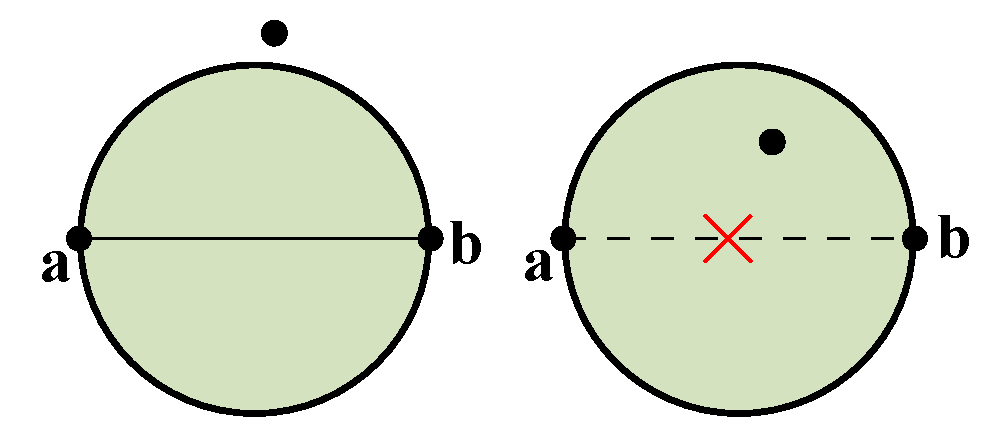
\includegraphics[width=0.45\textwidth]{gabriel.pdf}
    \caption{The two possible scenarios for the Gabriel graph. On the left side the points $a$ and $b$ are connected since the third point is outside the colored region. On the right side the third point is inside the region and the points $a$ and $b$ are disconnected.}
    \label{fig:gabriel}
\end{figure}
\begin{figure*}
    \centering
    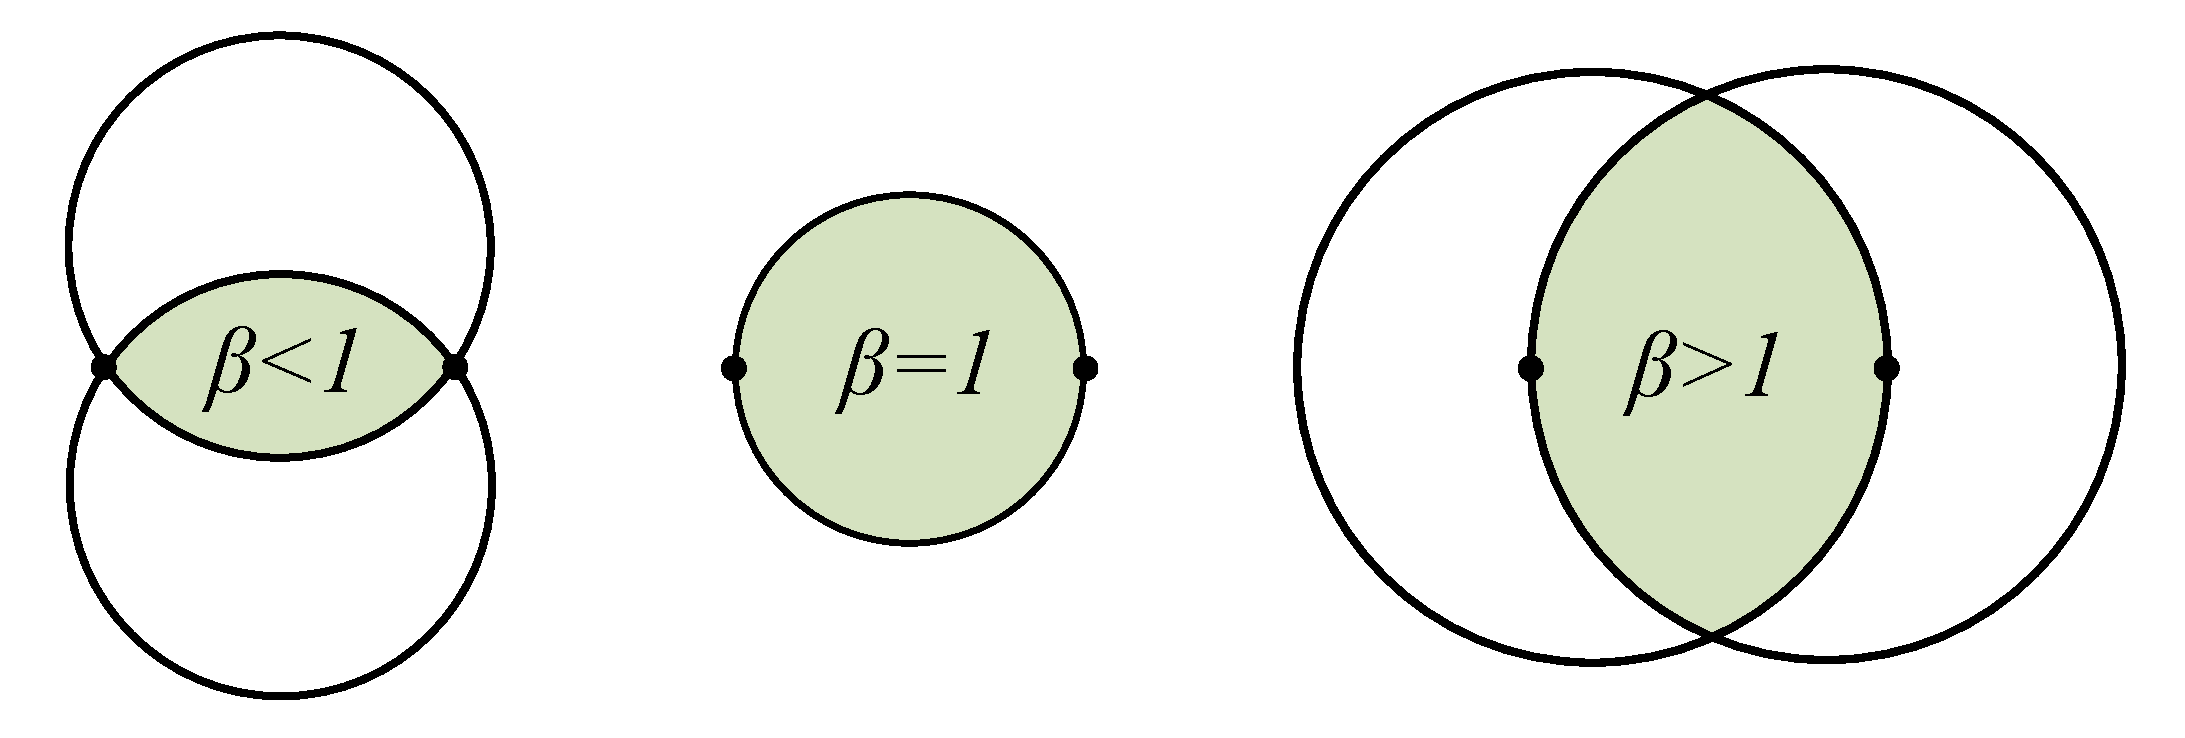
\includegraphics[width=0.9\textwidth]{betaskeleton.pdf}
    \caption{Exclusion region in the $\beta$-skeleton for different values of $\beta$. If beta is less than 1 the exclusion region is defined as the intersection between the two circles of radius $d/\beta$ that pass through the points. For beta larger than 1 the exclusion region is the intersection between the two circles with diameter $d\beta$ that pass through one of the points while the other lies on a diameter.}
    \label{fig:bskeleton_area}
\end{figure*}
\subsection{Graph Complexity Definition}

Once the graph is constructed the probability of a node having $n$ connections can be calculated as $p_n=N_{n}/T$. Where $N_{n}$ is the number of nodes with n connections and T is the total number of nodes. The next task is to find a scalar quantity that captures the structure of the graph. In this paper we have chosen the statistical complexity to be this quantity. One possible definition of complexity is found in \cite{lopez_comp}, where it is defined as:
\begin{equation}
	C(P)=S(P)D(P),
\end{equation}
where $S(P)$ is the Shannon entropy and
\begin{equation}
	D(P)=\sum_{n=1}^{N}\left(p_n - 1/N\right)^{2}.
\end{equation}
The motivation behind this type of definition is that it vanishes either if P has a well-defined outcome or if it is the uniform distribution.  Hence this definition is in agreement with the claim that pure randomness and pure certainty possess no structure. 
However, as it is shown in \cite{sig_com} it is more convenient to work with another definition of complexity:
\begin{equation}
    C(P)=\frac{D(P,U)H(P)}{D^{*}}.
    \label{eq:comp_def}
\end{equation}
where $H(P)$ is the normalized Shannon entropy, $D(P,U)$ is the Jensen-Shannon divergence between $P$ and the uniform distribution $U$,
\begin{equation}
	D(P,U)=S\left(\frac{P+U}{2}\right) - \frac{S(P)+S(U)}{2}.
\end{equation}
and $D^{*}$ is a normalization constant,
\begin{equation}
    D^{*}=-\frac{1}{2}\left[\frac{n+1}{n}\log_2(n+1)+\log_2(n)-2\log_2(2n)\right].
\end{equation}
Notice that the purpose of the Jensen-Shannon divergence is to make the complexity vanish whenever $P$ is the uniform. Hence, by computing this quantity with another distribution instead, we are changing what we consider to be a zero complexity distribution (apart from the delta-like distribution). The reason to change the definition of complexity once again shall become clear in the following sections.
\section{Methods}


\subsection{Simulations and Mock Catalogs}
The Abacus project \citep{abacus} is a set of N-body simulations of dark matter halos. It includes simulations with different box sizes and cosmological parameters. We use simulations of a cubic box of $720$\Mpch on each side with $1440^3$ particles. Each particle in the simulation has mass of $\sim1\times10^{10}$ \Msunh. The cube was simulated with 20 different initial conditions at standard cosmology and with 40 different cosmological parameters with the same initial conditions.
We build mock catalogs with two different geometries: spheres and spherical shells. In both cases the radius is $300$ \Mpch. The shells have an inner radius of $250$\Mpch. For every catalog we construct their random counterparts by randomizing the angular coordinates and fixing the radius. We also produced catalogs with and without Redshift Space Distortion (RSD) effects. To study the effect of redshift evolution we use spheres extracted from the snapshots at redshifts of $z=0.1$, $0.3$, $0.5$, $0.7$, $1$ and $1.5$.




\subsection{Numerical Experiments}

For each mock catalog we construct the $\beta$-skeleton and compute the probability of a node having $n$ connections $p_n$. From this distribution we calculate the complexity using equation \ref{eq:comp_def}. 

First we compare the complexity and entropy of a simulated sphere of points to that of a random sphere for $\beta$ between 1.0 and 5.0. The results found in this analysis motivate us to redefine our definition of complexity. The new equation is still basically \ref{eq:comp_def}, but now the Jensen-Shannon divergence is computed between the distribution of simulated points and the distribution of random points (not the uniform distribution). From now on we will use this definition.

We calculated the complexity for different values of $\beta$ and examined the influence of several variables on it. These variables were: cosmic variance, geometry, RSD, redshift evolution, cosmological parameters and number density.







\section{Results}
\label{sec:results}

Figure \ref{fig:cvb_viejo} shows the complexity as a function of $\beta$ for simulated and random points distributed within a sphere. There are two relevant things to underline. First, the complexity is not a continuous function of $\beta$. Second, the complexity of the random set of points is not zero or even close to zero compared to the simulated points. We found that the discontinuities of the complexity correspond to the values of $\beta$ for which the number of possible connections changes. For instance, at the discontinuity near $\beta$=4.0 the number of possible connections goes from 6 to 5. The second issue is easily explained since the random points do not generate a uniform distribution for the connections. Figures \ref{fig:svb} and \ref{fig:cvs_viejo} compare this definition of complexity to the Shannon entropy. We can see that the entropy, unlike the complexity, distinguishes between random and simulated points. 

Therefore, it is convenient to change the definition of complexity,
\begin{equation}
    C(P)=\frac{D(P,P_{random})H(P)}{D^{*}},
    \label{eq:comp_def2}
\end{equation}
where $P_{random}$ is the distribution of number of connections for the random points.

This new complexity, by construction, solves the problem of a random distribution having a complexity different from zero. Moreover, as shown in figure \ref{fig:cvb}, it turns out to be a smooth function of $\beta$ so fewer values of $\beta$ are needed. The complexity follows a decreasing tendency until it reaches its minimum value near $\beta$=3.3. The order of magnitude is $10^{-1}$ bits$^{2}$.

\subsection{Cosmic Variance}

We compare the complexity of 20 different spheres of standard cosmology built at $z=0.1$ without Redshift Space Distortions. Panel $a)$ in figure \ref{fig:4graf} shows the complexity of the 20 spheres with respect to one of them. From this plot it is easy to see that for $\beta$ 3.5 the complexity values are very similar. In fact, at this point the standard deviation is minimum (3.0$\times10^{-4}$ bits$^{2}$) and for $\beta$=1.0 it is maximum (3.1$\times10^{-3}$ bits$^{2}$). 



\subsection{Geometry}

We compare the complexity of 20 different spheres with that of 20 different spherical shells for standard cosmology,$z=0.1$, and no RSD. Panel $b)$ in figure \ref{fig:4graf} shows the mean complexity for the spheres and shells, as well as the standard deviation. For $\beta\leq3.0$ the complexity of the spheres is larger than that of the shells and are approximately equal afterwards. The difference between spheres and shells is of order $10^{-2}$ bits$^{2}$.




\subsection{Redshift Space Distortions}

We compare the complexity of 20 different spheres with and without RSD for standard cosmology and $z=0.1$. Panel $c)$ in figure \ref{fig:4graf} shows the mean complexity for both cases and the standard deviation. For $\beta\leq3.0$ the spheres with RSD have a bigger complexity than those without RSD and for $\beta\geq3.0$ the situation is the opposite. The differences between both cases is of order $10^{-2}$ bits$^2$.


\subsection{Redshift Evolution}
We compute the complexity for six values of redshift $z=$0.1, 0.3, 0.5, 0.7, 1.0, 15 without considering RSD. Panel $d)$ in figure \ref{fig:4graf} shows the evolution of complexity with $z$ for $\beta=$1.0, 1.5, 2.0, 2.5, 3.0. For each value of $\beta$ the complexity is taken with respect to the value at $z=0.1$. We see that for most values of $\beta$ there is an increasing tendency as $z$ gets larger. This is not the case for $\beta$=1.0, which falls rapidly between $z=1.0$ and $z=1.5$. The differences in complexity range from $10^{-2}$ to $10^{-3}$ bits$^2$.

\subsection{Cosmological Parameters}
We used the 40 different cosmologies available in the Abacus project to measure the influence on the complexity of the cosmological parameters $H_0$, $\Lambda$, $\Omega_{M}$, $n_s$, $\sigma_8$ and w$_0$. We calculated the complexity at $z=0.1$ without RSD and for $\beta$=1.0, 2.0, 3.5 and 5.0.  The Spearman’s rank correlation coefficient $\rho$ was used as a measure of correlation between $C$ and each one of the cosmological parameters. Figure \ref{fig:rhovb} shows $\rho$ as a function of $\beta$ for every cosmological parameter considered.  For most parameters the strongest correlation was found at $\beta$=5.0 and there was an abrupt change in the sign of $\rho$ from $\beta$=3.5 to 5.0. The exception was $n_{s}$ with the smallest correlation and variations with $\beta$. Figure \ref{fig:cvsigma8} shows the complexity for the 40 different values of $\sigma_{8}$ at $\beta=5.0$. This is the case with the strongest correlation, for which $\rho=0.511$.

\subsection{Number densities}
We compare the complexity of one sphere when different percentages of points are sampled. Figure \ref{fig:cvb_porcentaje} shows $C$ as a function of $\beta$ for every percentage considered. Although there are some exceptions, the complexity gets larger as one samples more and more points. The biggest changes are found at $\beta$=1.0 (maximum complexity) and the smallest ones at $\beta=3.5$ (minimum complexity). This is the most influential variable among the ones considered in this work as it has differences of the same order as the complexity ($10^{-1}$ bits$^2$).






\section{Conclusions}

In this paper we study several definitions of complexity to measure the structure of the cosmic web. We first construct the $\beta$-skeleton graph from N-body simulations and then compute the probability of a node having $n$ connections as $p_{n}=N_{n}/T$. It is on this distribution that our calculations are performed. We explore a definition proportional to the Shannon entropy and the Jensen-Shannon divergence between $P$ and the uniform distribution (eq. \ref{eq:comp_def}). This definition fails at assigning random distributions of points a complexity value different from zero and being a discontinuous function of $\beta$. We found that both issues can be solved by computing the Jensen-Shannon divergence with the probability distribution of a random set of points instead. This is due to the fact that random points do not have a uniform distribution of number of connections. 

We then study how this definition of complexity is affected by six factors: cosmic variance, geometry, Redshift Space Distortions (RSD), redshift evolution, cosmological parameters and number density. Cosmic variance turned out to be the least influential factor, with differences ranging from $10^{-4}$ to $10^{-3}$ bits$^2$. This means that the cosmic web is very homogeneous as far as complexity is concerned. The next factors are: cosmological parameters with changes of order $10^{-3}$ bits$^2$; redshift evolution (10$^{-3}$-10$^{-2}$); RSD (10$^{-2}$) and geometry (10$^{-2}$). The most influential factor is the number density with changes of the same order as the complexity ($10^{-1}$ bits$^2$) and a clear distinction between low and high number density. 

\section*{Acknowledgements}
XDL acknowledges the support from NSFC grant (No. 11803094).

\bibliographystyle{mnras}
\bibliography{references}

%\bsp	% typesetting comment
%\label{lastpage}
\begin{figure}
    \centering
    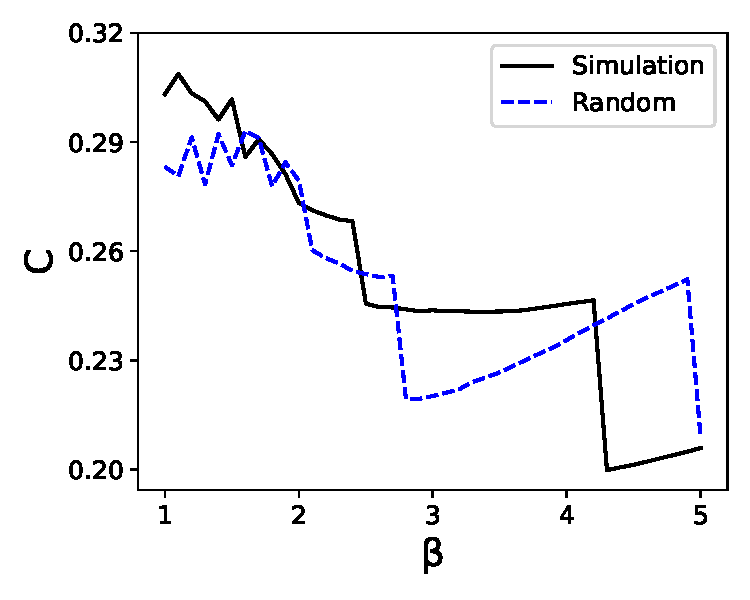
\includegraphics[width=0.45\textwidth]{cvb_viejo.pdf}
    \caption{First definition of complexity as a function of $\beta$ for random and simulated points.}
    \label{fig:cvb_viejo}
\end{figure}
\begin{figure}
    \centering
    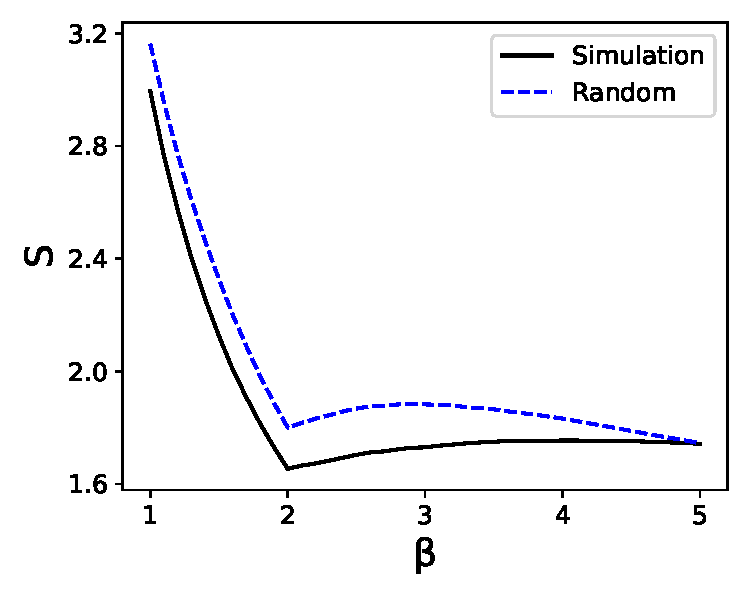
\includegraphics[width=0.45\textwidth]{svb.pdf}
    \caption{Entropy as a function of $\beta$ for random and simulated points.}
    \label{fig:svb}
\end{figure}
\begin{figure}
    \centering
    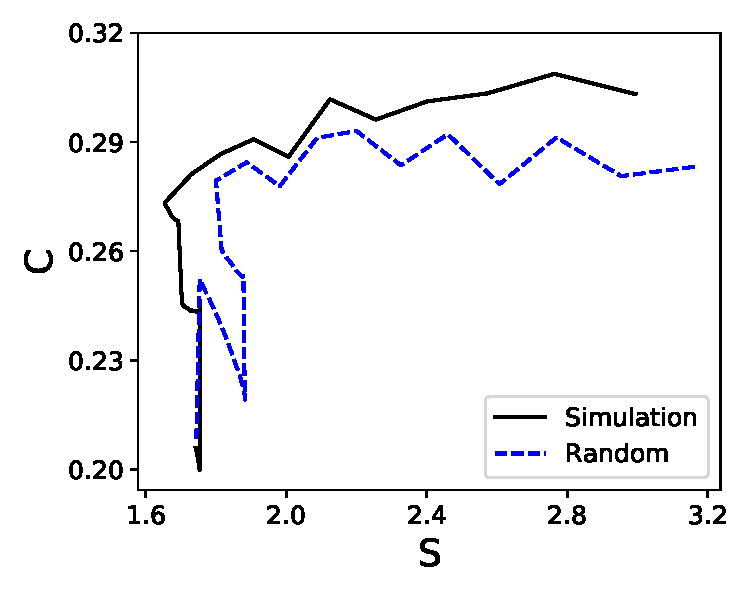
\includegraphics[width=0.45\textwidth]{cvs_viejo.pdf}
    \caption{First definition of complexity versus entropy for random and simulated points.}
    \label{fig:cvs_viejo}
\end{figure}
\begin{figure}
    \centering
    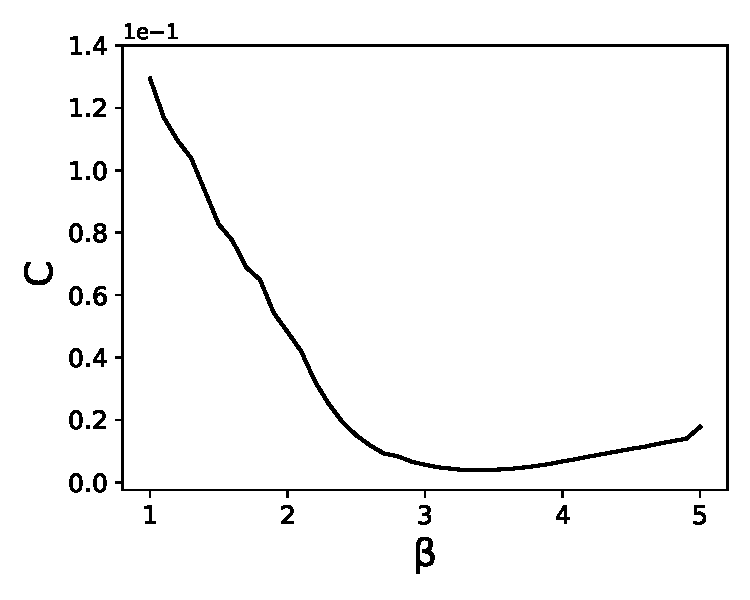
\includegraphics[width=0.45\textwidth]{cvb_inicial.pdf}
    \caption{Complexity as a function of $\beta$.}
    \label{fig:cvb}
\end{figure}
\begin{figure}
    \centering
    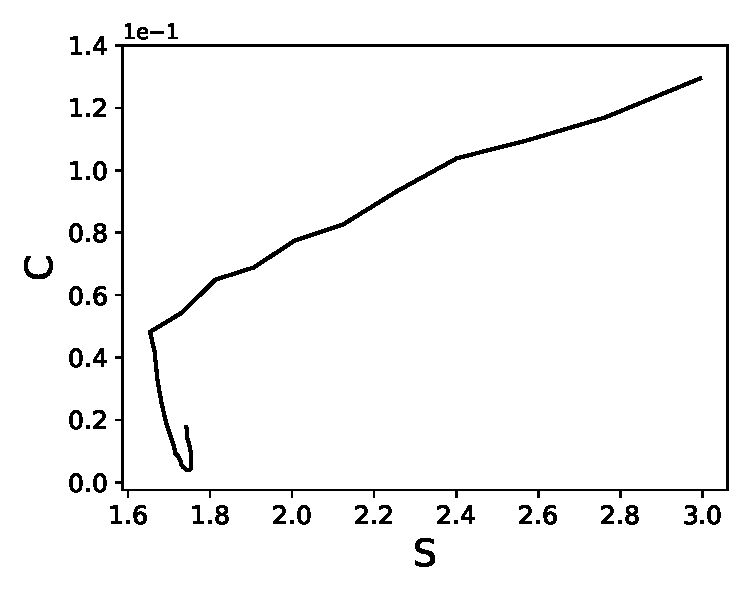
\includegraphics[width=0.45\textwidth]{cvs.pdf}
    \caption{Complexity versus entropy.}
    \label{fig:cvs}
\end{figure}
\begin{figure*}
    \centering
    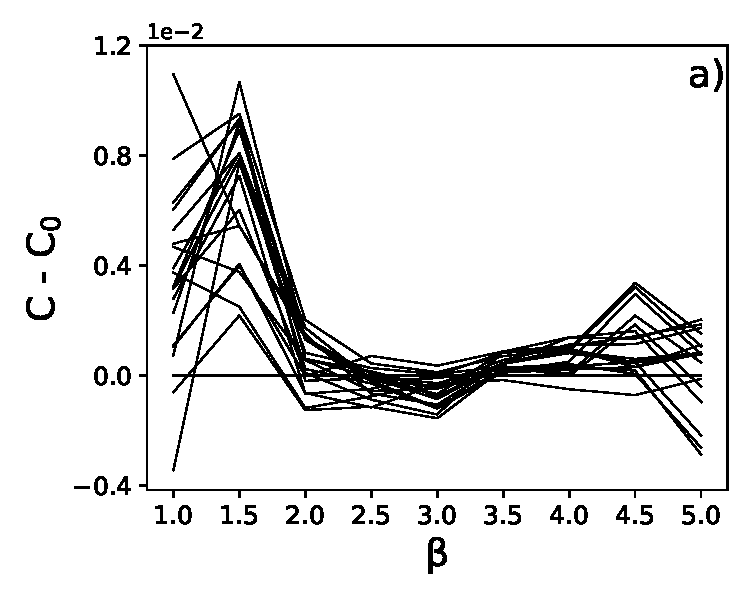
\includegraphics[width=0.4\textwidth]{varianza.pdf}
    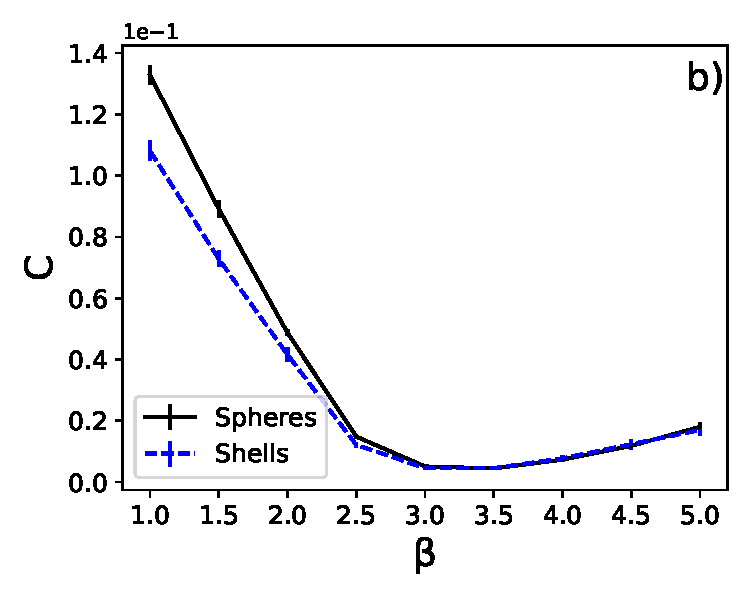
\includegraphics[width=0.4\textwidth]{geometria.pdf}
    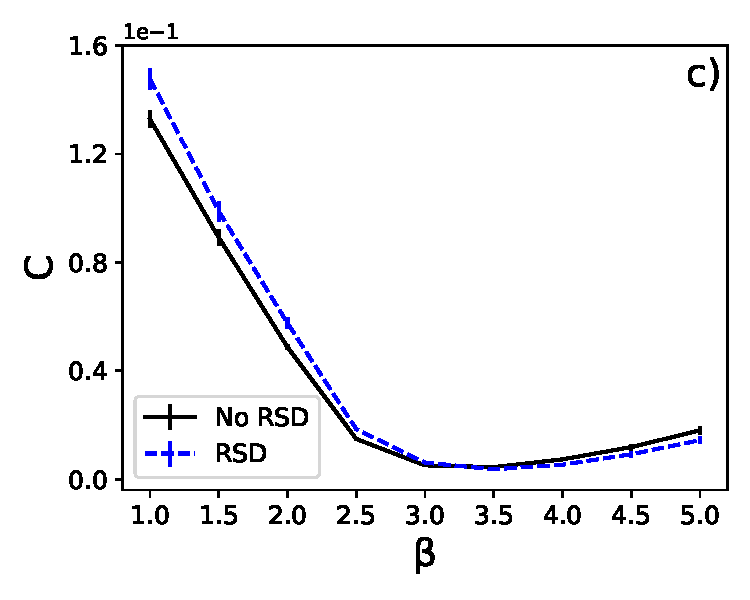
\includegraphics[width=0.4\textwidth]{rsd.pdf}
    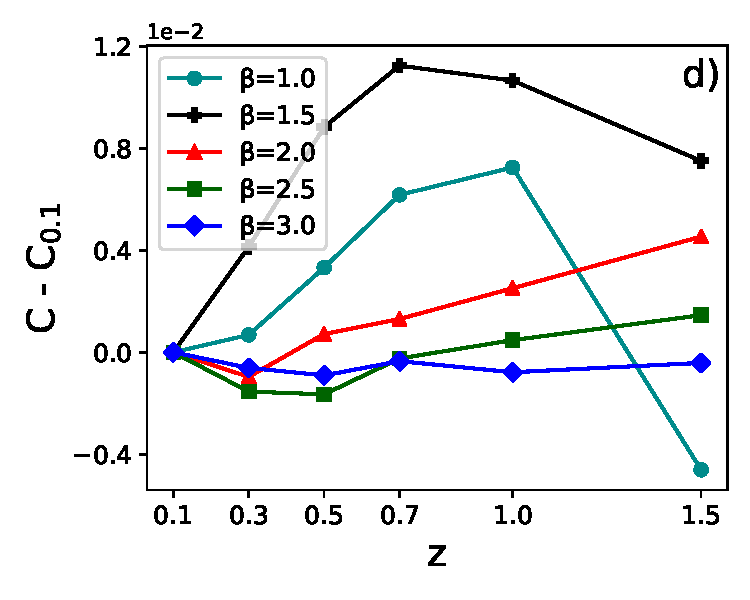
\includegraphics[width=0.4\textwidth]{rsd_evolution.pdf}
    \caption{a) Complexity as a function of $\beta$ for 20 spheres centered at different points. We plot the difference with respect to the complexity of one of the spheres $C_0$. b) Mean complexity as a function of $\beta$ for 20 spheres and shells centered at different points. The vertical lines represent the standard deviation. c) Mean complexity as a function of $\beta$ for 20 spheres, both considering redshift space distortions and not. The vertical lines represent the standard deviation. d) Complexity with respect to $z=0.1$ as a function of $z$ for 6 different values of $\beta$.}
    \label{fig:4graf}
\end{figure*}
\begin{figure}
    \centering
    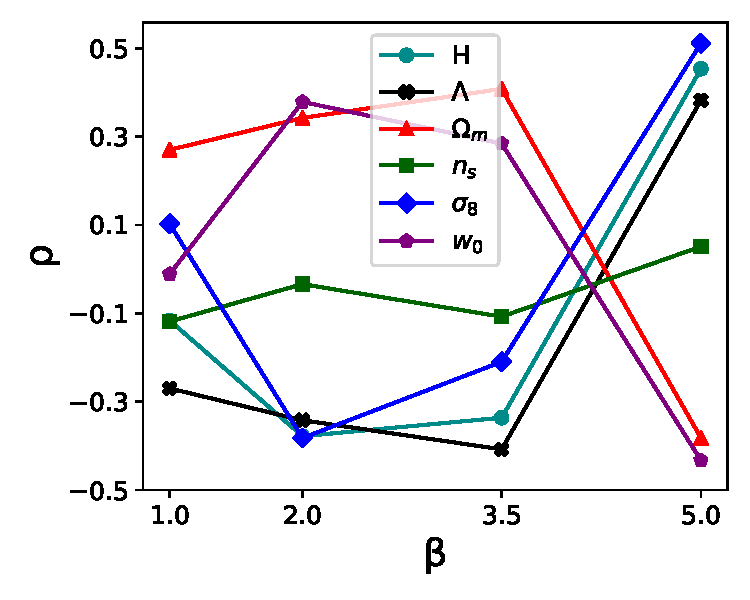
\includegraphics[width=0.45\textwidth]{rhovb.pdf}
\caption{Spearman's rank correlation coefficient between the statistical complexity and the cosmological parameters as a function of $\beta$.}
    \label{fig:rhovb}
\end{figure}
\begin{figure}
    \centering
    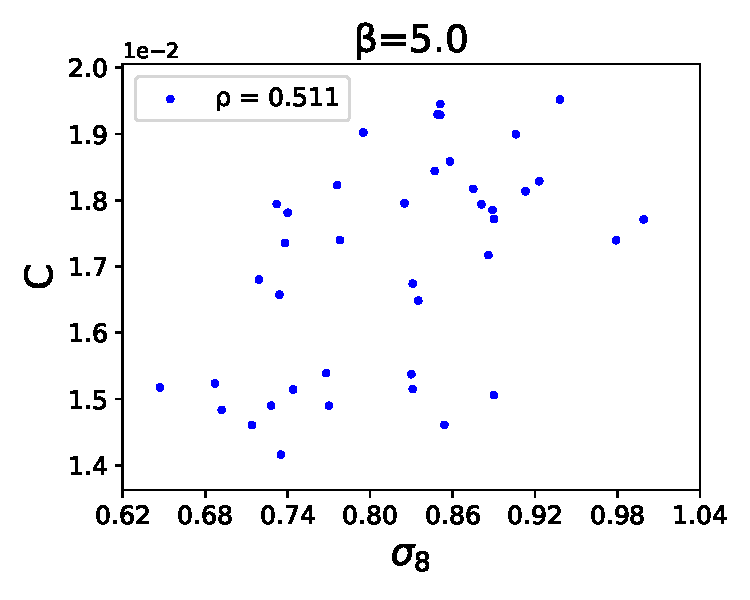
\includegraphics[width=0.45\textwidth]{cvsigma8.pdf}
    \caption{Complexity as a function of $\sigma_{8}$ for $\beta=5.0$. The Spearman's correlation coefficient is 0.511, the largest for the cosmological parameters considered.}
    \label{fig:cvsigma8}
\end{figure}
\begin{figure*}
    \centering
    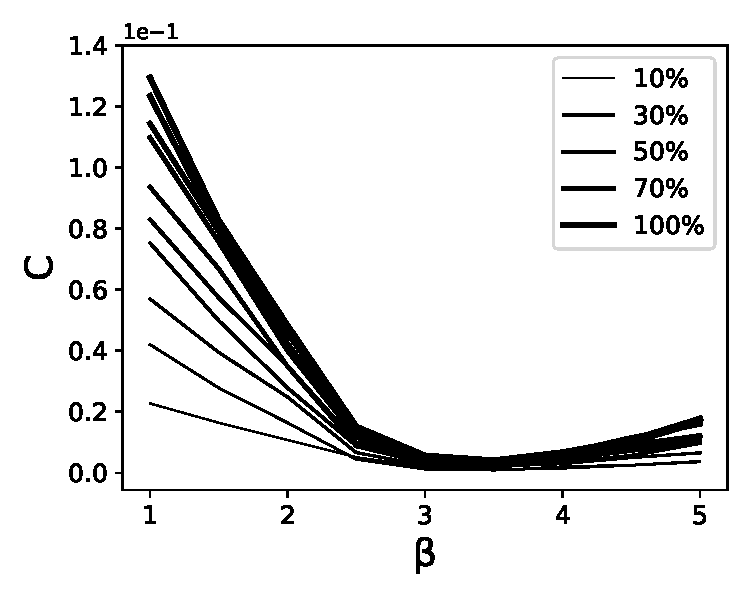
\includegraphics[width=0.9\textwidth]{cvb_porc.pdf}
    \caption{Complexity as a function of $\beta$ for several percentages of sampled points.}
    \label{fig:cvb_porcentaje}
\end{figure*}
\end{document}